\titlespacing*{\section}{0pt}{1.5\baselineskip}{2\baselineskip}
\titlespacing*{\subsection}{0pt}{1.5\baselineskip}{1\baselineskip}

\renewcommand{\sectionTitle}{Arquitectura de Software}
\section{\sectionTitle}
\label{sec:section3}

%4.1
\subsection{Edge AIoT Box}
\label{subsection:subsec3_1}

Este equipo realizara las siguientes funciones:

\begin{itemize}
    \item   Recopilar datos de un puerto habilitado de CANBUS J1939, interpretando los paquetes de datos y 
            filtrar los datos deseados de todos los disponibles
    \item   Almacenarlos dentro de una base de datos para facilitar su manejo y consultas.
    \item   Habilitar un puerto de enlace Wifi con un servidor HTML para consultar los datos de la base de datos.
    \item   Un sistema que evalúa el estado de la batería externa del sistema y realiza acciones correspondientes.
\end{itemize}

\begin{figure}[H]
    \centering
    \includegraphics[height=2in]{images/edge_arquitectura.png}
    \captionsetup{font=footnotesize}
    \caption{Arquitectura de Software - Edge AIoT Box}
    \label{fig:img2}
\end{figure}

%4.2
\subsection{Nodo Portable}
\label{subsection:subsec3_2}

Este equipo realizara las siguientes funciones

\begin{itemize}
    \item   Realizar consultas al Web Server del Edge AIoT Box 
            para obtener los datos almacenados de este equipo mediante su Módem interno.
    \item   Almacenar dichos datos en una tarjeta SD incorporada en el Nodo Portable
    \item   Enviar estos datos almacenados en una SD hacia la nube usando su Módem interno
    \item   Registrar datos del nivel de batería del equipo Nodo Portable
\end{itemize}

\begin{figure}[H]
    \centering
    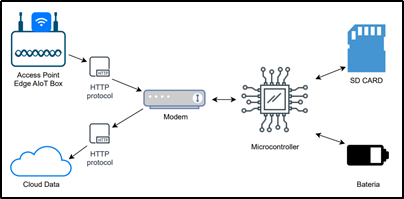
\includegraphics[height=2in]{images/nodo_arquitectura.png}
    \captionsetup{font=footnotesize}
    \caption{Arquitectura de Software - Nodo Portable}
    \label{fig:img3}
\end{figure}

